%% =============================================================================
%% Relatório final de atividades -- Bolsa de Doutoramento FCT 2021.04591.BD
%% Ricardo Barbosa Sousa -- PDEEC/FEUP -- INESC TEC (CRIIS/iiLab)
%%
%% Compilação: latexmk -pdf main.tex   (pdflatex + biber)
%%
%% Campos por confirmar marcados com \tbc{...} (aparecem a vermelho no PDF).
%% Para os encontrar: grep -n "tbc{" main.tex
%% =============================================================================
\documentclass[11pt,a4paper,oneside]{article}

%% ---------------------------------------------------------------------------
%% PACOTES
%% ---------------------------------------------------------------------------
\usepackage[T1]{fontenc}
\usepackage[utf8]{inputenc}
\usepackage[portuguese]{babel}
\IfFileExists{XCharter.sty}{\usepackage[osf]{XCharter}}{\usepackage{charter}}

\usepackage{microtype}
\usepackage[a4paper,top=3cm,bottom=3cm,left=1.5cm,right=1.5cm,
            headheight=14pt,footskip=1cm]{geometry}
\usepackage{graphicx}
\usepackage[table]{xcolor}
\usepackage{booktabs}
\usepackage{tabularx}
\usepackage{array}
\usepackage{enumitem}
\usepackage{fancyhdr}
\usepackage{titlesec}
\usepackage{pdflscape}
\usepackage{afterpage}
\usepackage{pgfgantt}
\usepackage{siunitx}
\usepackage{amsmath}
\usepackage{csquotes}
\usepackage[backend=biber,
            style=numeric,
            sorting=ynt,
            sortcites=true,
            defernumbers=true,
            giveninits=true,
            maxbibnames=99,
            minbibnames=99,
            maxcitenames=2,
            url=false,
            isbn=false,
            eprint=false]{biblatex}
\usepackage[hidelinks]{hyperref}
\usepackage{xurl}
\usepackage{pdfpages}

%% ---------------------------------------------------------------------------
%% CONFIGURAÇÃO
%% ---------------------------------------------------------------------------
\addbibresource{references.bib}
\graphicspath{{figures/}}
\urlstyle{same}

% Nomes do \autoref em português europeu
\addto\extrasportuguese{%
  \def\sectionautorefname{Secção}%
  \def\subsectionautorefname{Secção}%
  \def\tableautorefname{Tabela}%
  \def\figureautorefname{Figura}%
}

% Prefixos das referências: [C#] contributos da tese, [P#] outras publicações
\assignrefcontextkeyws[labelprefix=C]{core}
\assignrefcontextkeyws[labelprefix=P]{other}

% Campos por confirmar
\newcommand{\tbc}[1]{\textcolor{red}{[#1]}}

\sisetup{
  output-decimal-marker = {,},
  group-separator       = {\,},
  per-mode              = symbol
}

\definecolor{fctblue}{RGB}{0,45,70}
\definecolor{bargray}{gray}{0.55}
\definecolor{planfill}{RGB}{214,220,228}
\definecolor{planedge}{gray}{0.55}

\setlist{nosep,leftmargin=*}
\setlist[itemize]{label=\textbullet,topsep=3pt,itemsep=2pt}

\titleformat{\section}{\Large\bfseries}{\thesection}{0.8em}{}
\titleformat{\subsection}{\large\bfseries}{\thesubsection}{0.8em}{}
\titlespacing*{\section}{0pt}{1.6em}{0.8em}
\titlespacing*{\subsection}{0pt}{1.2em}{0.5em}

\setlength{\parindent}{1.5em}
\setlength{\parskip}{0.2em}
\linespread{1.08}

%% Dados do relatório -------------------------------------------------------
\newcommand{\bolsaref}{2021.04591.BD}
\newcommand{\bolsadoi}{10.54499/2021.04591.BD}
\newcommand{\bolsatitulo}{RicoSLAM: Long-Term Localization and Mapping in Dynamic Environments}
\newcommand{\tesetitulo}{RicoSLAM: Localization and Mapping in Dynamic Environments}
\newcommand{\autor}{Ricardo Barbosa Sousa}
\newcommand{\datarelatorio}{19 de outubro de 2026}

%% Rodapé de financiamento --------------------------------------------------
% Para usar os logótipos oficiais (barra FCT / República Portuguesa / etc.),
% colocar o ficheiro figures/logos-financiamento.pdf; caso contrário é
% impressa a menção textual.
% \newcommand{\rodapefinanciamento}{%
%   \IfFileExists{figures/logos-financiamento.pdf}{%
%     \includegraphics[width=\textwidth]{logos-financiamento.pdf}%
%   }{%
%     \parbox{\textwidth}{\centering\footnotesize\color{black!60}%
%       Bolsa de doutoramento \bolsaref{} financiada por fundos nacionais através da\\
%       Fundação para a Ciência e a Tecnologia (FCT)%
%       ~(DOI:~\href{https://doi.org/\bolsadoi}{\bolsadoi})}%
%   }%
% }
%
% Logótipos: figures/logo-republica-portuguesa.png e figures/logo-fct.png
% (versão positiva, a preto, com fundo transparente).
\newcommand{\rodapefinanciamento}{%
  \parbox{\textwidth}{\centering
    \raisebox{-0.5\height}{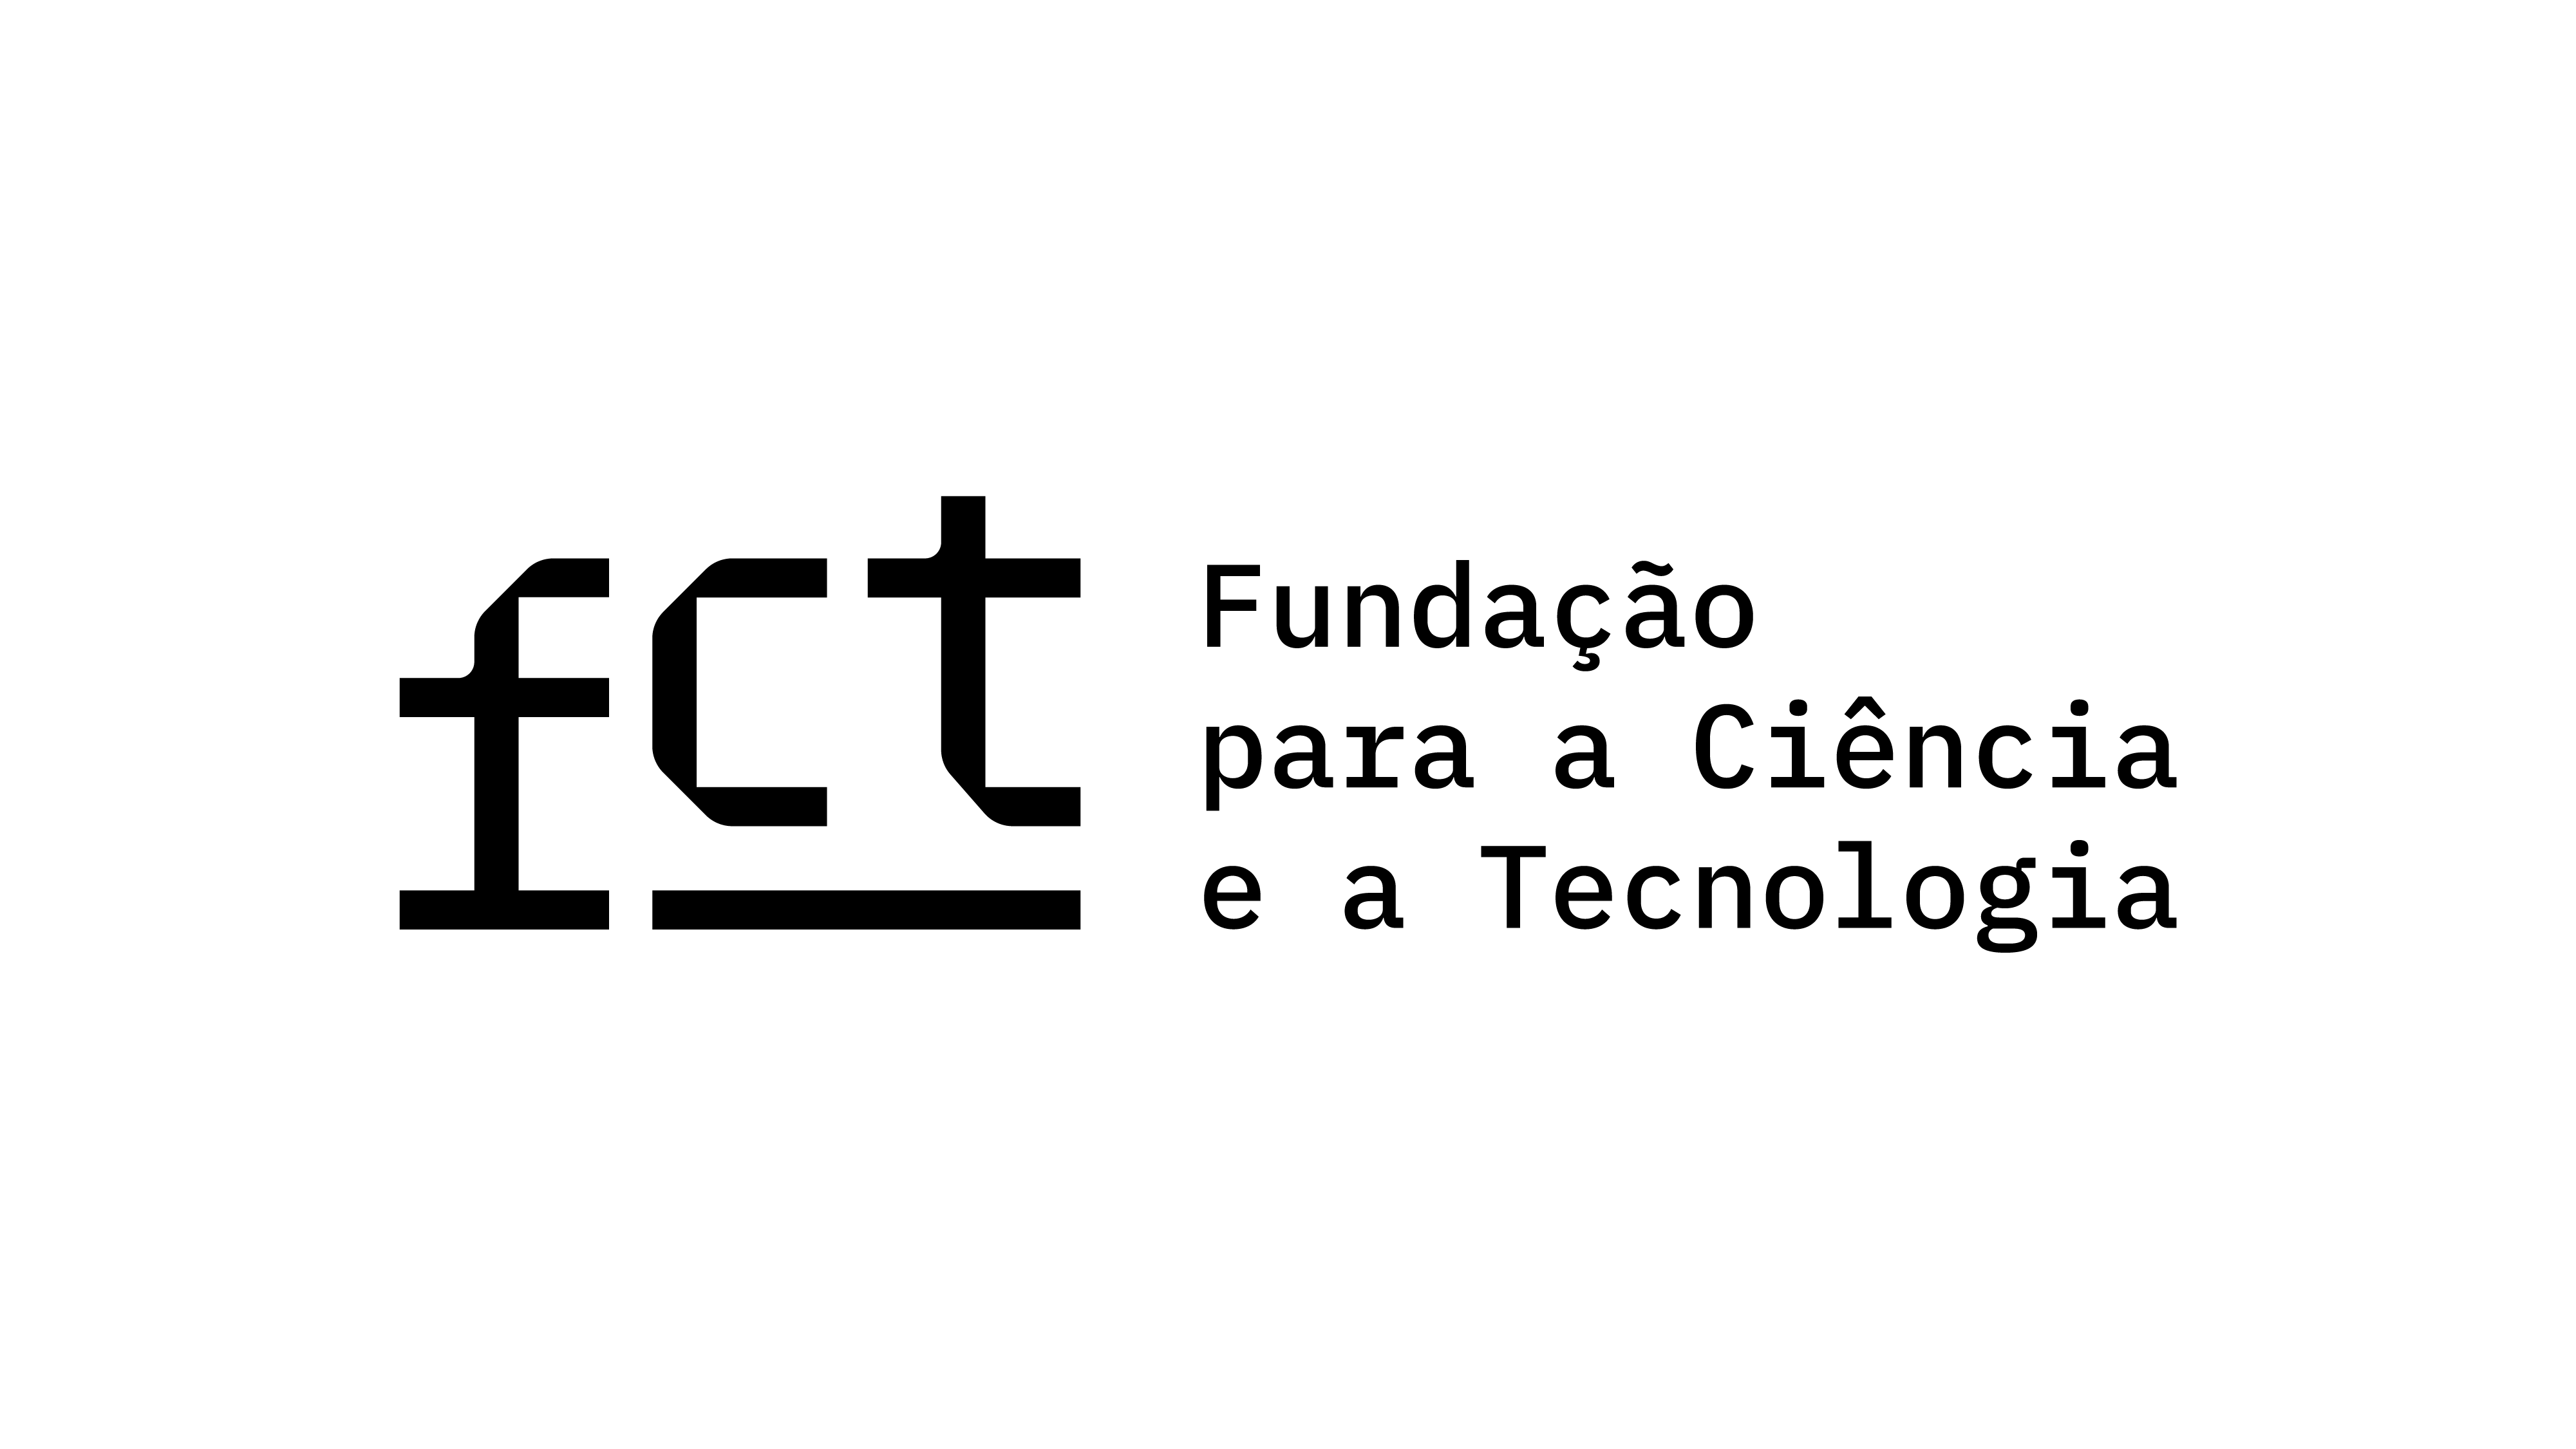
\includegraphics[height=1.20cm]{logo-fct.png}}%
    \raisebox{-0.5\height}{
\includegraphics[height=1.20cm]{logo-republica-portuguesa.png}}%
    \hspace{0.50cm}%
    \raisebox{-0.5\height}{
\includegraphics[height=1.20cm]{logo-greenauto.png}}%
    \hspace{0.50cm}%
    \raisebox{-0.5\height}{
\includegraphics[height=1.20cm]{logo-prr.png}}%
  }%
}

\pagestyle{fancy}
\fancyhf{}
\renewcommand{\sectionmark}[1]{\markright{\thesection\ #1}}
\fancyhead[L]{\small\itshape\rightmark}
\fancyhead[R]{\small\thepage}
\fancyfoot[C]{\rodapefinanciamento}
\renewcommand{\headrulewidth}{0pt}
\fancypagestyle{plain}{%
  \fancyhf{}%
  \fancyfoot[C]{\rodapefinanciamento}%
  \renewcommand{\headrulewidth}{0pt}%
}

%% Título da secção de referências
\defbibheading{subbib}[\bibname]{\subsection*{#1}}

\hypersetup{
  pdftitle    = {Relatório de atividades -- Bolsa FCT \bolsaref},
  pdfauthor   = {\autor},
  pdfsubject  = {\bolsatitulo},
  pdfkeywords = {SLAM, robótica móvel, ambientes dinâmicos, laser 2D}
}

%% =============================================================================
\begin{document}
%% =============================================================================

%% ---------------------------------------------------------------------------
%% CAPA
%% ---------------------------------------------------------------------------
\begin{titlepage}
\thispagestyle{plain}
\centering
\vspace*{0.4cm}
{\large\bfseries\scshape Fundação para a Ciência e a Tecnologia\par}
\vspace{2.0cm}
{\huge\bfseries RicoSLAM: Long-Term Localization and\\[0.25em] Mapping in Dynamic Environments\par}
\vspace{1.2cm}
{\large\bfseries \autor\par}
\vspace{1cm}
{\large\scshape Bolsas de Doutoramento 2021\par}
{\large \bolsaref\par}
{\small DOI:~\href{https://doi.org/\bolsadoi}{\bolsadoi}\par}
\vspace{1.5cm}

\includegraphics[height=1.55cm]{uporto-feup.pdf}\hspace{1.4cm}%
\raisebox{0.35cm}{
\includegraphics[height=0.95cm]{inesctec.png}}\par
\vspace{1cm}
{\large Programa Doutoral em Engenharia Eletrotécnica e de Computadores\par}
\vspace{1cm}
\begin{minipage}{\textwidth}
\setlength{\parskip}{0.6em}
\raggedright
{\normalsize Orientador: Professor Doutor António Paulo Gomes Mendes Moreira.}\\
{\small Professor Catedrático do Departamento de Engenharia Eletrotécnica e de
Computadores da Faculdade de Engenharia da Universidade do Porto.\\
Investigador no Centro de Robótica Industrial e Sistemas Inteligentes
(CRIIS) do INESC TEC -- Instituto de Engenharia de Sistemas e Computadores,
Tecnologia e Ciência.\par}
{\normalsize Coorientador: Doutor Héber Miguel Sobreira.}\\
{\small Investigador no Centro de Robótica Industrial e Sistemas Inteligentes
(CRIIS) do INESC TEC -- Instituto de Engenharia de Sistemas e Computadores,
Tecnologia e Ciência.\par}
\end{minipage}
\vfill
{\normalsize \datarelatorio\par}
{\normalsize \copyright{} \autor, 2026}
\vspace{1cm}
\end{titlepage}

%% ---------------------------------------------------------------------------
%% ÍNDICE
%% ---------------------------------------------------------------------------
\renewcommand{\contentsname}{Conteúdo}
\tableofcontents
\clearpage

%% ===========================================================================
\section{Contextualização}\label{sec:contexto}
%% ===========================================================================

O objetivo deste relatório é reportar as atividades desenvolvidas e os resultados
obtidos no âmbito da bolsa de doutoramento \bolsaref{}
(DOI:~\href{https://doi.org/\bolsadoi}{\bolsadoi}), concedida pela Fundação para
a Ciência e a Tecnologia~(FCT) a \autor, com início a 1 de setembro de
2021 e suspensa a 31 de março de 2023, possibilitando a obtenção do grau de
Doutor no Programa Doutoral em Engenharia Eletrotécnica e de Computadores (PDEEC)
a setembro de 2026, com a tese intitulada de \enquote{\tesetitulo}, sob a
orientação do Professor Doutor António Paulo Gomes Mendes Moreira e a
coorientação do Doutor Héber Miguel Sobreira.

A instituição de acolhimento para a execução das atividades desenvolvidas no
âmbito da bolsa concedida pela FCT e na tese de doutoramento foi o INESC TEC --
Instituto de Engenharia de Sistemas e Computadores, Tecnologia e Ciência, onde
todo o trabalho foi realizado no iiLab -- Industry and Innovation Laboratory e no
Centro de Robótica Industrial e Sistemas Inteligentes~(CRIIS).
Em abril de 2023, o bolseiro suspendeu a sua bolsa de investigação concedida pela
FCT para transitar para um contrato de investigação no INESC TEC no âmbito da
Agenda GreenAuto -- \textit{Green Innovation for the Automotive Industry},
mais concretamente, no PPS18 -- \textit{3D navigation system for mobile robotic
equipment} do WP10 -- \textit{automated logistics for the automotive industry},
liderado pela Flowbotic Mobile Systems. O restante trabalho de doutoramento foi
realizado ao abrigo do PPS18 até à sua conclusão.
Com isto, o presente relatório cobre a totalidade do trabalho de doutoramento.

A tese aborda o problema da localização e mapeamento simultâneos
(\textit{Simultaneous Localization and Mapping}, SLAM) de robôs móveis autónomos
(\textit{Autonomous Mobile Robots}, AMR) em ambientes interiores dinâmicos,
em particular industriais e de intralogística, recorrendo a dados de
\textit{lasers}~2D e, opcionalmente, à odometria das rodas possibilidade pela
leitura dos encoders dos motores.
Estes ambientes contêm elementos em movimento (pessoas, outros veículos) e sofrem
reconfigurações ao longo do tempo (paletes, caixas, máquinas), o que degrada a
consistência do mapa e a estimativa da pose do robô.
O trabalho foi orientado por duas questões de investigação~(QI):
\begin{itemize}
\item \textbf{QI1:} como melhorar os resultados de mapeamento ao realizar SLAM
      com um robô móvel terrestre num ambiente interior dinâmico?
\item \textbf{QI2:} como integrar a dinâmica do ambiente no processo de
      localização ao realizar SLAM nas mesmas condições?
\end{itemize}

%% ===========================================================================
\section{Atividades curriculares}\label{sec:curricular}
%% ===========================================================================

O PDEEC da FEUP tem um total de 240 ECTS num período de quatro anos, que são
distribuídos entre a componente das Unidades Curriculares (60~ECTS) no primeiro
ano e a execução dos trabalhos e apresentação da Tese de Doutoramento (180~ECTS)
nos restantes anos curriculares. A \autoref{tab:ucs} lista as unidades
curriculares frequentadas e as respetivas classificações finais.

\begin{table}[ht]
\centering
\caption{Lista de unidades curriculares e classificações finais.}
\label{tab:ucs}
\begin{tabular}{@{} p{0.6\linewidth} ccc@{}}
\toprule
\textbf{Unidade curricular} & \textbf{Ano} & \textbf{ECTS} & \textbf{Classificação final} \\
\midrule
Manipuladores Robóticos                                                                        & 1 &   6   & 18 \\
Plano de Tese                                                                                  & 1 &  18   & 19 \\
Robótica Móvel                                                                                 & 1 &   6   & 19 \\
Seminários: Publicação e Escrita Científica                                                    & 1 &   3   & 18 \\
Seminários: Competências Transversais para Engenharia -- Gestão do Tempo e Organização Pessoal & 1 &   1.5 & 19 \\
Seminários: Competências Transversais para Engenharia -- Métodos de Investigação Científica    & 1 &   1.5 & 17 \\
Tópicos Avançados Engenharia Eletrotécnica e de Computadores                                   & 1 &   6   & 17 \\
Tópicos Especiais                                                                              & 1 &  12   & 19 \\
Visão Computacional                                                                            & 1 &   6   & 17 \\
Tese                                                                                           & 2 & 180   & Aprovado \\
Tese                                                                                           & 3 & 180   & Aprovado \\
Tese                                                                                           & 4 & 180   & Aprovado \\
\bottomrule
\end{tabular}
\end{table}

A tese foi submetida a 17 de junho de 2026 e aprovada em provas públicas de
doutoramento realizadas a 18 de setembro de 2026, pelas 14h, na sala I025 do
Departamento de Engenharia Eletrotécnica e de Computadores~(DEEC) da FEUP.
O júri da prova pública foi composto pelos seguintes elementos:
Doutor José Nuno Moura Marques Fidalgo (Presidente), Professor Associado com
Agregação do DEEC da FEUP;
Doutora Milena Faria Pinto (Vogal), Professora do Centro Federal de Educação
Tecnológica Celso Suckow da Fonseca, Rio de Janeiro, Brazil;
Doutor Robert Henry Deaves (Vogal), \textit{Honorary Professor at the Deparment
of Mechanical Engineering of the College of Engineering and Physical
Sciences~(EPS) at the University of Birmingham, UK};
Doutor Carlos Baptista Cardeira (Vogal), Professor Associado do Departamento de
Engenharia Mecânica do Instituto Superior Técnico da Universidade de Lisboa;
Doutor Paulo José Cerqueira Gomes da Costa (Vogal), Professor Associado do DEEC
da FEUP; e Doutor António Paulo Gomes Mendes Moreira~(Orientador), Professor
Catedrático do DEEC da FEUP.
A versão final da tese de doutoramento foi entregue nos
Serviços Académicos da FEUP a 25 de setembro de 2026.

%% ===========================================================================
\section{Trabalho desenvolvido}\label{sec:trabalho}
%% ===========================================================================

O cronograma proposto originalmente na candidatura respetiva à bolsa  \bolsaref
~está representado na \autoref{fig:gantt} (barras claras), a par da execução
efetiva dos trabalhos (barras escuras). A proposta consistia em dividir o
trabalho de investigação em onze tarefas ao longo de 48~meses, entre fevereiro de
2021 e janeiro de 2025, tarefas as quais são descritas de seguida:
\begin{enumerate}[label=\arabic*.,leftmargin=2em]
\item Tarefa~1 (\textit{Curricular plan and literature research}): plano
      curricular e revisão de literatura;
\item Tarefa~2 (\textit{Calibration of the sensory systems}): calibração dos
      sistemas sensoriais;
\item Tarefa~3 (\textit{Evaluation of SLAM algorithms from the literature}):
      avaliação de algoritmos de SLAM da literatura;
\item Tarefa~4 (\textit{Data acquisition}): aquisição de dados;
\item Tarefa~5 (\textit{Architecture of the system}): arquitetura do sistema;
\item Tarefa~6 (\textit{Simulation environment}): ambiente de simulação;
\item Tarefa~7 (\textit{SLAM algorithm}): algoritmo de SLAM;
\item Tarefa~8 (\textit{Persistence algorithm for mapping purposes}): algoritmo
      de persistência para mapeamento;
\item Tarefa~9 (\textit{Fault detection algorithms}): algoritmos de deteção de
      falhas;
\item Tarefa~10 (\textit{Tests and validation}): testes e validação;
\item Tarefa~11 (\textit{Paper submission reviews and thesis writing}):
      submissão e revisão de artigos e escrita da tese.
\end{enumerate}

%% CRONOGRAMA (plano vs. execução) -------------------------------------------
%% Plano: datas exatas da candidatura. Execução: aproximada (ver comentários).
%% Formato das datas: aaaa-mm.
%% ---------------------------------------------------------------------------
\newcommand{\gplan}[3]{\ganttbar[bar/.append style={fill=planfill, draw=planedge, line width=0.4pt},
  bar top shift=0.14, bar height=0.32]{#1}{#2}{#3}}
\newcommand{\gexec}[2]{\ganttbar[bar/.append style={fill=fctblue, draw=none},
  bar top shift=0.52, bar height=0.32]{}{#1}{#2}}
\newcommand{\gmile}[1]{\ganttmilestone[milestone/.append style={fill=black, draw=white, line width=0.5pt},
  milestone top shift=0.50, milestone height=0.36]{}{#1}}

\afterpage{%
\begin{landscape}
\begin{figure}[p]
\centering
\caption{Cronograma do plano original da candidatura (barras claras, em cima)
e da execução efetiva (barras escuras, em baixo). Os losangos assinalam a
publicação ou aceitação dos resultados de cada tarefa:
T1~\cite{sousa:jfr:2023};
T2~\cite{sousa:jint:2022};
T3~\cite{ribeiro:access:2025};
T4~\cite{sousa:icarsc:2025} e~\cite{ribeiro:dataset:2025};
T7~\cite{sousa:icara:2024} e~\cite{sousa:robot:2026};
T10~\cite{lopes:icara:2026};
T11, submissão da tese e provas públicas.
A linha a tracejado vermelho marca o fim previsto do plano original da
bolsa proposto em face de candidatura (janeiro de 2025).}
\label{fig:gantt}
\vspace{0.4em}
\resizebox{\linewidth}{!}{%
\begin{ganttchart}[
    time slot format = isodate-yearmonth,
    time slot unit   = month,
    x unit           = 2.75mm,
    y unit title     = 6.5mm,
    y unit chart     = 7.6mm,
    title height     = 1,
    hgrid            = {*1{black!12}},
    vgrid            = {*{11}{draw=none}, *1{black!30, dashed}},
    bar label font          = \small,
    bar inline label node/.append style = {font=\scriptsize\bfseries, text=white},
    milestone label font    = \small,
    title/.append style     = {fill=fctblue, draw=none},
    title label font        = \small\bfseries\color{white},
    canvas/.append style    = {draw=black!25},
    vrule/.style            = {very thick, red!75!black, dashed},
  ]{2021-01}{2026-12}
  \gantttitlecalendar{year} \\
  %
  %
  \gplan{T1. Plano curricular e revisão da literatura}{2021-02}{2022-01}
    \gexec{2021-02}{2023-01}  % plano de tese (TRP) defendido a 12/01/2023
    \gmile{2023-04} \\        % SLR publicada a 11/04/2023
  %
  %
  \gplan{T2. Calibração dos sistemas sensoriais}{2022-01}{2022-04}
    \gexec{2022-01}{2022-06}  % somente em termos de trabalhos experimentais neste âmbito
    \gmile{2022-06} \\        % OptiOdom publicado a 08/06/2022
  %
  %
  \gplan{T3. Avaliação de algoritmos de SLAM}{2022-03}{2022-05}
    \gexec{2022-06}{2026-05}  % lab tests + visiting research + continuous evaluation of SLAM algorithms
    \gmile{2025-12} \\        % IILABS 3D SLAM benchmark article
  %
  %
  \gplan{T4. Aquisição de dados}{2022-03}{2023-02}
    \gexec{2022-06}{2024-12}  % 5dpo MSL + Hangfa + IDEPA + ...
    \gmile{2025-02}           % Dataset IILABS 3D público
    \gmile{2025-04} \\        % Modified Hangfa Discovery Q2 ICARSC paper
  %
  %
  \gplan{T5. Arquitetura do sistema}{2022-06}{2022-06}
    \gexec{2023-01}{2024-07} \\ % features (possível arquitetura) + visiting research period
  %
  %
  \gplan{T6. Ambiente de simulação}{2022-02}{2022-05}
    \gexec{2024-02}{2024-12} \\ % benchmarks sintéticos (registo e GBA), stage_ros
  %
  %
  \gplan{T7. Algoritmo de SLAM}{2022-07}{2023-02}
    \gexec{2023-01}{2026-03}  % features, mapas de distância e RicoSLAM
    \gmile{2024-02}           % detetor (ICARA, 02/2024)
    \gmile{2026-09} \\        % ROBOT2026 aceite em 09/2026
  %
  %  
  \gplan{T8. Persistência no mapeamento}{2022-10}{2023-12}
    \gexec{2024-05}{2026-03} \\ % remoção de dinâmica por ray tracing (online e offline)
  %
  %
  \gplan{T9. Deteção de falhas}{2023-07}{2024-04} \\
  %
  %
  \gplan{T10. Testes e validação}{2023-03}{2024-10}
    \gexec{2023-07}{2026-07}  % validação em cinco datasets, com cartographer
    \gmile{2026-02} \\        % CARGO (ICARA 2026, 02/2026)
  %
  %
  \gplan{T11. Artigos e escrita da tese}{2022-02}{2025-01}
    \gexec{2022-02}{2026-09}
    \gmile{2026-06}           % submissão tese
    \gmile{2026-09} \\[grid]  % prova pública 18/09/2026
  %
  \ganttbar[bar/.append style={fill=black!35, draw=none}, bar top shift=0.2,
    bar height=0.6, inline, bar inline label node/.append style={text=black}]%
    {Bolsa FCT}{2021-09}{2023-03}
  \ganttbar[bar/.append style={fill=black!65, draw=none}, bar top shift=0.2,
    bar height=0.6, inline]%
    {Contrato INESC TEC (GreenAuto, PPS18)}{2023-04}{2026-09}
  \ganttbar[bar label font=\small\bfseries, bar/.style={draw=none, fill=none}]%
    {Financiamento}{2021-01}{2021-01} \\
  \ganttbar[bar/.append style={fill=black!65, draw=none}, bar top shift=0.2,
    bar height=0.6, bar label font=\small\bfseries]%
    {Estadia na Sapienza (não prevista)}{2024-02}{2024-07}
  %
  \ganttvrule{}{2025-01}
\end{ganttchart}%
}

\vspace{0.6em}
\begin{tikzpicture}[font=\footnotesize]
  \filldraw[fill=planfill, draw=planedge, line width=0.4pt] (0,0) rectangle (0.6,0.2);
  \node[anchor=west] at (0.7,0.1) {Plano da candidatura};
  \fill[fctblue] (4.2,0) rectangle (4.8,0.2);
  \node[anchor=west] at (4.9,0.1) {Execução efetiva};
  \fill[black] (8.0,0.1) -- (8.1,0.26) -- (8.2,0.1) -- (8.1,-0.06) -- cycle;
  \node[anchor=west] at (8.3,0.1) {Publicação, aceitação ou marco};
  \draw[very thick, red!75!black, dashed] (13.6,-0.06) -- (13.6,0.26);
  \node[anchor=west] at (13.75,0.1) {Fim previsto do plano};
\end{tikzpicture}
\end{figure}
\end{landscape}
}

As tarefas T1, T3, T4, T5, T7, T10 e T11 foram concluídas. As tarefas T2 e T6
foram concluídas parcialmente, a T8 foi concluída com o âmbito revisto e a T9
não foi executada como tarefa isolada. A tese foi submetida a 17 de junho de
2026, 17~meses depois do fim previsto do plano.
Os fatores que contribuiram para este desvio do plano original foram a suspensão
da bolsa em abril de 2023, com a transição para um contrato de investigação no
INESC~TEC no âmbito do PPS18 da Agenda GreenAuto, e a estadia de seis meses na
Sapienza Università di Roma em 2024 com o Doutor Giorgio Grisetti, não prevista
na candidatura, que esteve na origem dos contributos centrais da segunda parte da
tese relativos ao desenvolvimento do algoritmo SLAM. Em consequência, as
tarefas T7, T8 e T10 decorreram sobretudo entre 2024 e 2026. Quanto ao âmbito,
a tese restringiu-se a dados de \textit{lasers} 2D e, opcionalmente, de
odometria das rodas, focando-se na configuração habitual dos AMR na logística,
ao invés de de explorar fusão de odometria, câmaras, \textit{lasers} e
IMU prevista na candidatura.

O trabalho do doutoramento foi distribuído pela publicação de vários artigos
científicos. No total, resultaram da tese oito contributos~[C1--C8]: dois
artigos em revistas científicas, três artigos em conferências internacionais,
um artigo aceite para publicação, um manuscrito em preparação e um
\textit{dataset} público.

Na Tarefa~1, para além do plano curricular (\autoref{sec:curricular}), foi
realizada uma revisão sistemática da literatura sobre SLAM com plataformas móveis
em operações a longo prazo, que incluiu 142~trabalhos e resultou no artigo
\enquote{A systematic literature review on long-term localization and mapping for
mobile robots}~\cite{sousa:jfr:2023}, publicado no
\textit{Journal of Field Robotics}.

Na Tarefa~2, a calibração da odometria das rodas resultou no artigo
\enquote{OptiOdom: a generic approach for odometry calibration of wheeled mobile
robots}~\cite{sousa:jint:2022}, contributo originado da dissertação de mestrado
do bolseiro \autor. A calibração extrínseca foi abordada apenas
através da indexação dos sensores pelo desenho CAD da plataforma
experimental~\cite{sousa:icarsc:2025} e das sequências de calibração incluídas
no \textit{dataset} IILABS~3D~\cite{ribeiro:dataset:2025}, ou então assumindo-se
que os parâmetros extrínsecos eram conhecidos nos datasets usados na tese.
No entanto, os desenvolvimentos no contexto de correção da pose offline pela
framework RicoSLAM demonstraram o potencial do uso da mesma como ground-truth
para a posição do sensor laser~2D, possibilitando a exploração de calibração
simultânea e automática dos parâmetros extrínsecos e da odometria de rodas em
robôs móveis industriais.

Das Tarefas~3 e~4 resultaram a modificação da plataforma Hangfa Discovery~Q2
para integrar perceção multimodal, descrita no artigo \enquote{Integrating
multimodal perception into ground mobile robots}~\cite{sousa:icarsc:2025}, o
\textit{dataset} público IILABS~3D~\cite{ribeiro:dataset:2025} e o artigo
\enquote{Indoor benchmark of 3-D LiDAR SLAM at iilab -- industry and innovation
laboratory}~\cite{ribeiro:access:2025}, que avalia algoritmos de SLAM da
literatura sobre esse \textit{dataset}. Foram ainda reunidas sequências de AMR
em ambientes industriais e académicos (Avantgarde, Cappero, Flowbotic e Kuka).

Nas Tarefas~5 e~6, a arquitetura final do sistema SLAM foi definida durante a
estadia na Sapienza, com um \textit{front-end} de registo e um \textit{back-end}
de otimização do grafo de poses com o srrg2\_solver. Para além disso, foi
explorada uma arquitetura do sistema SLAM compatível com a extração de features
dos dados do laser~2D. Em vez de um ambiente de simulação completo, foram
desenvolvidos \textit{benchmarks} sintéticos para o registo de nuvens de pontos e
para a otimização global. No entanto, o simulador Stage foi usado e adaptado na
tese, inclusive adicionando wrappers para ROS~2, para validação da framework
RicoSLAM.

Da Tarefa~7 resultaram o artigo \enquote{Line fitting-based corner-like detector
for 2D laser scanners data}~\cite{sousa:icara:2024}, o artigo \enquote{Unsigned
distance maps on 2D point cloud registration}~\cite{sousa:robot:2026}, aceite na
ROBOT2026, e a \textit{framework} RicoSLAM, descrita no manuscrito
\enquote{RicoSLAM: framework for localization and mapping in dynamic
environments}~\cite{sousa:ral:2026}, em preparação para a \textit{IEEE Robotics
and Automation Letters}.

Na Tarefa~8, em vez de algoritmos de aprendizagem, a distinção entre
observações dinâmicas e estáticas foi concretizada por um mecanismo de remoção
de dinâmica baseado em \textit{ray tracing}, que opera \textit{online}, na
atualização dos mapas locais, e \textit{offline}, na geração do mapa de ocupação
final~\cite{sousa:ral:2026}.
Esta mudança de implementação teve como intuito a framework RicoSLAM ser capaz
de lidar com ambientes industriais altamente dinâmicos e não perder a localização
durante o processo de mapeamento, mas também permitir gerar uma representação do
ambiente mais limpa em termos de observações estáticas, melhorando a operação a
longo prazo de robôs móveis autónomos industriais.

A Tarefa~9 não foi executada como tarefa autónoma e isolada. Os contributos mais
próximos estão integrados no próprio sistema: a rejeição de
\textit{loop closures} com baixa proporção de \textit{inliers} e uma métrica de
consistência do registo que aumenta quando o alinhamento falha numa direção
degenerada.

No âmbito da Tarefa~10, o RicoSLAM foi validado no IILABS~3D e nas sequências
industriais e académicas, obtendo o menor erro absoluto de trajetória nas quatro
sequências planares do IILABS~3D face ao GMapping e ao SLAM~Toolbox. O sistema
foi também usado numa aplicação de descarga de contentores, descrita no artigo
\enquote{CARGO: container-unloading autonomous robot with generalized
operation}~\cite{lopes:icara:2026}.

Por fim, na Tarefa~11, a tese foi submetida a 17 de junho de 2026 e aprovada em
provas públicas a 18 de setembro de 2026.

%% ===========================================================================
\section{Mobilidade internacional}\label{sec:mobilidade}
%% ===========================================================================

Entre fevereiro e julho de 2024, foi realizada uma estadia de investigação de
seis meses na Sapienza Università di Roma, sob a supervisão do Professor Doutor
Giorgio Grisetti, junto do Robotics Vision and Perception Group (RVP-Group) e do
LabRoCoCo do Department of Computer, Control and Management Engineering (DIAG).
A estadia, inicialmente prevista para três meses, foi prolongada para seis
meses. Da colaboração resultaram os contributos centrais da segunda parte da
tese: a \textit{framework} de registo baseada em mapas de distância, a
\textit{framework} RicoSLAM e a formulação de \textit{Global Bundle
Adjustment}~(GBA) baseada em mapas de distância,
em coautoria com o Professor Doutor Giorgio Grisetti~\cite{sousa:robot:2026,
sousa:ral:2026}. A estadia permitiu ainda o acesso direto ao srrg2\_solver,
adotado como \textit{back-end} do RicoSLAM, e às sequências Cappero e Kuka,
usadas na avaliação da remoção de dinâmica com dados reais.

%% ===========================================================================
\section{Participação em eventos}\label{sec:eventos}
%% ===========================================================================

Durante a execução da tese de doutoramento, houve participação nas seguintes
conferências e eventos:
\begin{itemize}
\item ICARA 2024 -- 10\textsuperscript{th} International Conference on
      Automation, Robotics and Applications, em Atenas, Grécia, com o artigo
      \cite{sousa:icara:2024};
\item ICARSC 2024 -- IEEE International Conference on Autonomous Robot Systems
      and Competitions, em Paredes de Coura, com o artigo
      \cite{sousa:icarsc:2024};
\item ICARSC 2025, no Funchal, com os artigos
      \cite{sousa:icarsc:2025,pacheco:icarsc:2025,lopes:icarsc:2025};
\item ROBOT2026 -- 9\textsuperscript{th} Iberian Robotics Conference, em
      Barcelona, Espanha, para a apresentação do artigo aceite
      \cite{sousa:robot:2026};
\item várias edições da competição Robot@Factory~4.0 do Festival Nacional de
      Robótica, com a equipa de robótica 5dpo da FEUP.
\end{itemize}

%% ===========================================================================
\section{Outras atividades}\label{sec:outras}
%% ===========================================================================

\paragraph{Docência.} Assistente Convidado na FEUP entre 2021 e 2023.

\paragraph{Coorientação.} No 2.\textsuperscript{o} semestre de 2022/23, foram
coorientados cinco estudantes de licenciatura (quatro da FEUP e um do ISEP) em
temas ligados à tese: localização e mapeamento com a plataforma Hangfa
Discovery~Q2 e com uma plataforma omnidirecional de três rodas, controlo de
trajetória de robôs omnidirecionais, compensação da distorção de movimento em
dados de \textit{lasers} 2D e avaliação experimental de algoritmos de SLAM com
LiDAR 3D. Foram ainda coorientados cinco bolseiros de iniciação à investigação
(BII) no INESC TEC, em deteção de paletes para ambientes intralogísticos, deteção
de caixas metálicas para o setor automóvel e teleoperação de AMR sobre redes 5G.

\paragraph{Projetos de I\&D.} Para além da Agenda GreenAuto, houve participação
nos projetos PRODUTECH~R3, VINCI~7D e 5G \& Digital Transformation Test Bed.
Desta participação, e da colaboração com a equipa 5dpo da FEUP, resultaram as
publicações \cite{sousa:icarsc:2021,sousa:jint:2022,sousa:access:2022,
caldana:robot:2024,levin:robot:2024}, para além das já referidas na
\autoref{sec:eventos}.

%% ===========================================================================
\section{Publicações e resultados}\label{sec:resultados}
%% ===========================================================================

O trabalho apresentado coincide com a publicação de oito contributos no âmbito
da tese~[C1--C8]: dois artigos em revistas científicas internacionais (\textit{Journal
of Field Robotics} e \textit{IEEE Access}), três artigos em atas de conferências
internacionais (ICARA 2024, ICARSC 2025 e ICARA 2026), um artigo aceite para
publicação (ROBOT2026), um manuscrito em preparação para a \textit{IEEE Robotics
and Automation Letters} e um \textit{dataset} público, o
IILABS~3D~\cite{ribeiro:dataset:2025}, disponível no repositório de dados do
INESC TEC. No mesmo período, foram publicados outros oito artigos~[P1--P8],
dois em revistas e seis em conferências internacionais.

Como resultado da tese, foram ainda disponibilizados os seguintes repositórios
de \textit{software} aberto ao público:
\begin{itemize}
\item \url{https://github.com/INESCTEC/ricoslam}: \textit{framework} RicoSLAM
      completa;
\item \url{https://github.com/INESCTEC/inesctec_mrdt_line_fit_based_corner_detector_2d_laser}:
      implementação C++, compatível com ROS~1, do detetor de características
      em \textit{lasers} 2D~\cite{sousa:icara:2024};
\item \url{https://github.com/INESCTEC/inesctec_mrdt_hangfa_discovery_q2}:
      documentação e código das modificações à plataforma Hangfa Discovery~Q2,
      com página pública em \url{https://oss.inesctec.pt/inesctec_mrdt_hangfa_discovery_q2/}~\cite{sousa:icarsc:2025};
\item \url{https://github.com/sousarbarb/slr-ltlm-mr}: documentação, dados e
      \textit{scripts} da revisão sistemática~\cite{sousa:jfr:2023};
\item \url{https://github.com/sousarbarb/hector_slam} e
      \url{https://github.com/sousarbarb/slam_gmapping}: nós \textit{offline}
      adicionados ao Hector~SLAM e ao GMapping para processar múltiplos
      ficheiros ROS \textit{bag} e exportar trajetórias no formato TUM;
\item \url{https://github.com/sousarbarb/stage_ros}: \textit{wrapper} ROS do
      simulador Stage, compatível com ROS~1 e ROS~2;
\item \url{https://gitlab.com/sousarbarb_srrg-software/srrg_system}:
      compatibilidade CMake com ROS~1 e ROS~2 dos pacotes srrg2\_core,
      srrg2\_qgl\_viewport e srrg2\_solver.
\end{itemize}

%% ---------------------------------------------------------------------------
%% REFERÊNCIAS
%% ---------------------------------------------------------------------------
\section*{Referências}
\addcontentsline{toc}{section}{Referências}
\markright{Referências}

\begin{refcontext}[labelprefix=C]
\printbibliography[keyword=core,heading=subbib,title={Contributos da tese}]
\end{refcontext}

\begin{refcontext}[labelprefix=P]
\printbibliography[keyword=other,heading=subbib,title={Outras publicações no período do doutoramento}]
\end{refcontext}

%% ---------------------------------------------------------------------------
%% ANEXOS
%% ---------------------------------------------------------------------------
\clearpage
\appendix
\includepdf[pages=-,
            addtotoc={1,section,1,Certidão e ata das provas de doutoramento,anexo:ata}]%
           {20260929-161014.pdf}

%% ---------------------------------------------------------------------------

\end{document}
